
% \begin{frame}{Future work}

% Note that there was no talk of correct specification for the
% data you have.

% That was a foregone conclusion when we started looking at equivalent weights!

% How do you peform model checking with sensitivity analysis?

% Existing methods evaluate whether the analysis changes ``a lot'' when you:
% %
% \begin{itemize}
% \item Parametrically perturb the model (e.g.~fit a richer model class)
% \item Non--parameterically perturb the data (e.g.~produce gross outliers)
% \end{itemize}
% %
% The problem is:
% %
% \begin{itemize}
% \item How much is ``a lot''?
% \item Non--parametric data perturbations are hard to reason about
% \item It's hard to say whether parametric model changes are enough
% \end{itemize}
% %


% Instead, we
% %
% \begin{itemize}
% \item Parametrically perturb the data
% \item Observe whether our model could detect the change
% \end{itemize}
% %
% \begin{itemize}
% \item Know exactly the expected change (don't have to decide on what ``a lot'' means)
% \item Easy to reason about whether the data perturbation is reasonable
% \item Don't need to propose an alternative model, instead study the model you have
% \end{itemize}


% \end{frame}

\begin{frame}{Future work}

Notice that there was no discussion of misspecification!\\[1em]

\emph{Calibration weights (typically) do not depend on $\Ysur$.}

\pause

\vspace{2em}
But the high level idea can be extended much more widely:
%
\begin{enumerate}
\item Assume your initial model was accurate
\item Select some perturbation your model should be able to capture
\item Use local sensitivity to detect whether the change is what you expect
\item If the change is not what you expect, either (1) or (2) was wrong
\end{enumerate}
%

\pause

\vspace{2em}
Such checks recover generlized versions of many standard diagnostics for linear models.\\[1em]
Examples:
\begin{itemize}
\item Additive parameter shifts $\quad\leftrightarrow\quad$ Unbiasedness
\item Invariance to survey data weighting $\quad\leftrightarrow\quad$ Regressor + residual orthogonality
\item Importance sampling $\quad\leftrightarrow\quad$ Sandwich covariance $\overset{?}{=}$ Inverse Fisher information
\end{itemize}

\vspace{2em}


\end{frame}


%%%%%%%%%%%%%%%%%%%%%%%%%%%%%%%%%%%%%%%%
%%%%%%%%%%%%%%%%%%%%%%%%%%%%%%%%%%%%%%%%
%%%%%%%%%%%%%%%%%%%%%%%%%%%%%%%%%%%%%%%%


\begin{frame}{Future work}

Student contributions and ongoing work:

\begin{itemize}
% \item \textbf{Alice Cima} contributed significantly to this work
\item \textbf{Vladimir Palmin} is working on extending MrPlew to \texttt{lme4}
\item \textbf{Sequoia Andrade} is working on generalizing to other local sensitivity checks
\item \textbf{Lucas Schwengber} is working on novel flow--based techniques for local sensitivity
\item \textbf{(Currently recruiting!)} Doubly--robust Bayesian Hierarchical MrP
\end{itemize}


{
    \centering
% \begin{minipage}[t]{0.24\textwidth}
%     \centering
%     
\includegraphics[width=0.9\textwidth]{static_figures/alice.jpg}\\
%     Alice Cima
% \end{minipage}
\begin{minipage}[t]{0.24\textwidth}
    \centering
    
\includegraphics[height=0.9\textwidth]{static_figures/vladimir_palmin.jpg}\\
    Vladimir Palmin
\end{minipage}
\begin{minipage}[t]{0.24\textwidth}
    \centering
    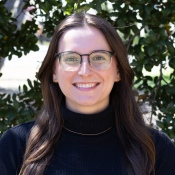
\includegraphics[height=0.9\textwidth]{static_figures/sequoia.jpg}\\
    Sequoia Andrade
\end{minipage}
\begin{minipage}[t]{0.24\textwidth}
    \centering

\includegraphics[height=0.9\textwidth]{static_figures/lucas.jpg}\\
Lucas Schwengber
\end{minipage}

}

\hrulefill

\textbf{Preprint and \texttt{R} package (hopefully) coming soon!}


\end{frame}

%%%%%%%%%%%%%%%%%%%%%%%%%%%%%%%%%%%%%%%%
%%%%%%%%%%%%%%%%%%%%%%%%%%%%%%%%%%%%%%%%
%%%%%%%%%%%%%%%%%%%%%%%%%%%%%%%%%%%%%%%%


